\documentclass[fontsize=11pt]{article}
\usepackage{amsmath}
\usepackage[utf8]{inputenc}
\usepackage[margin=0.75in]{geometry}
\usepackage{hanging}
\usepackage{hyperref}
\usepackage{graphicx}

\title{CSC110 Project Report: The Effect of Climate Change on Flooding Susceptibility in Coastal Regions (Vancouver Area)}
\author{Lorena Buciu, Kevin Yang, Ricky Yi, Rafee Rahman}
\date{Monday, December 14, 2020}

\begin{document}
    \maketitle

    \section*{Introduction}

    \textbf{How has climate change affected the sea levels in the Vancouver area over the years? Based on this, which areas project to be susceptible to flooding 280 years in the future?} \\

    Climate change has a number of devastating impacts on the environment. One of the issues that arise as a result of climate change is the global acceleration of sea-level rise. Sea-level rise (SLR), measured in metres, is frequently observed by researchers and has been known to be increasing for years. Changes in global temperature result in glaciers melting as well as the warming of ocean water, causing it to become less dense and expand, overall resulting in sea-level rise (Hausfather, 2019). Coastal regions are most heavily impacted by these changes since an increased sea-level will begin to take up land and potentially endanger those living nearby and increase the risk of floods and damage to agricultural land. Sea-level rise also has implications for inland areas since the displacement of civilians would mean an increased impact on even non-coastal regions. \\

    A study from Nature Communications finds that approximately 300 million people live in areas at risk of flooding (Kulp \& Strauss, 2019). Countries including China, Bangladesh, and Vietnam are already facing heavy floods due to sea-level rise. Based on sea-level projections for 2050, land in these areas will fall below the elevation threshold for annual coastal floods (Jennings, 2019). Therefore, it is important to predict when in the future the sea-levels in those areas will pose a risk to those people if we do not slow down the effects of climate change. \\

    The goal of our research is to predict and visualize the effects of sea-level changes due to climate change in coastal regions, focusing on the greater Vancouver area. We have decided to analyze areas along the coastline to determine which are most at risk of flooding in the future by comparing the estimated future sea-level to the elevation of coastal regions. According to the 2016 Census, Vancouver has one of the highest population densities in Canada, so climate change and, by extension, SLR puts the many people living there at risk. Researchers are also worried that sea-level rise in this region may be 3 times worse than expected (Kulp \& Strauss, 2019).


    \section*{Dataset Description}

    \hspace{\parindent}A dataset that we have used is from the NOAA / NESDIS / Laboratory for Satellite Altimetry Website. It is a CSV file that contains the sea level change in the north pacific ocean, given in millimetres. This file is named pacificocean\_sea\_level.csv. \\

    The data ranges from the year 1992 to 2020  (there are multiple satellite captures for each year) and the values were obtained by the TOPEX/Poseidon, Jason-1, Jason-2, and Jason-3 satellites. The dataset contains 4 columns, one for the year, and 3 for each satellite and the value that it recorded at a point during the year. An example of data that is in this dataset is: A capture during the year 2020 by the Jason-3 satellite is a change of 140.61mm. \\

    We have cleaned this CSV dataset by calculating the mean sea level change for each year instead of having multiple captures for one year, putting all the satellite data together, and using this data we can predict the change in future years. We created a new CSV file called data\_predictions.csv that contains two columns for the year and the corresponding sea level, including the values we predicted with our Theil-Sen regression model. \\

    Another dataset we have used is Vancouver surface elevation data from the Topographic Information section of the Government of Canada website. It is an ASC file (but we can easily read it as a .txt file) that contains digital surface model (DSM) data based on a selected area of the Vancouver region we are analyzing. The value 0 in this dataset represents the elevation at sea level. We can compare this elevation data to the sea level data so that we can determine flooding susceptibility. This data was interpreted into a grid of latitude and longitude values through calculations which allowed us to plot the data points on a plotly mapbox. \\

    After interpreting this DSM data, the program will create a new CSV file called below\_sea\_level.csv which contains all of the points which are below the given sea level for a certain year. This file contains 3 columns, latitude, longitude, and elevation. \\

    The program also creates a dataset named sarimax\_model\_data.csv, necessary for displaying the SARIMAX prediction model. This dataset has two columns, year (contains dates as datetime.datetime objects) and the \texttt{mean\_sea\_level} predicted by that model. \\

    \section*{Computational Plan}
    \textbf{Part 1: Data Cleaning}

    \hspace{\parindent}Our program is mainly composed of two parts, data processing and then extrapolation. With the datasets being in CSV and ASC format, we needed to read them while at the same time removing any unnecessary data not needed for calculations. Most of these operations are done in the \texttt{data\_cleaning.py} file. In this file we use the \texttt{csv} module to access the contents of the files then use a combination of for loops and module features from pandas and numpy to mutate our data so that it is compatible with our calculation functions. This is perhaps best demonstrated by the \texttt{read\_csv\_data()} function in the \texttt{data\_cleaning.py} file. This function aims to transform our pacificocean\_sea\_level.csv file into a dictionary \texttt{Dict[str, List[Tuple[str, float]]]} that will work with the rest of the program. To do this, it filters out empty values from the base data set and appends usable data points into the return dictionary. \\

    A major computation performed by our program to transform this new data is seen in the \texttt{group\_means()} function, also found in the \texttt{data\_cleaning.py} file. This function iterates through this newly created dictionary, extracting the years from each satellite and computing the means, resulting in a formatted dictionary by mutation done by the helper function  \texttt{remove\_dupes()} with the years as the keys mapping to the mean sea level for that year. This condenses our original pacificocean\_sea\_level.csv into a simpler, summarized dataset. The program will write our transformed data into a new CSV file called predicted\_data.csv for pandas compatibility later on which is done through the usage of the \texttt{csv} module. \\

    The most important data processing is seen in the \texttt{canada\_dsm.py} file. This file interprets the elevation\_data.asc file into latitude and longitude points which will be plotted into our map visualization. This file achieves this mainly through the \texttt{assign\_coords()} function. The original elevation\_data.asc file contains values for the number of rows, columns, latitude of the bottommost coordinate, longitude of the leftmost coordinate, and the cell size. Using these initial values, we can use a nested for loop and some calculations to interpret each elevation into a latitude and longitude coordinate, based on its position in an ascii grid. \\


    \textbf{Part 3: Reporting Results}

    \hspace{\parindent}As described in the introduction, the main form of reporting takes the form of an interactive map of the Vancouver area. Based on the extrapolated values we computed, the user of our program is able to move a slider to select a year and the extrapolated results will be displayed on a map. There is also another slider which allows the user to select a sea level and see which areas are going to be affected by that selected sea level. The dash framework allowed us to establish an interactive front-end visualization, using HTML and dash core components to program a dynamic slider. \\

    To determine which points are below the given sea level, we have the \texttt{check\_elevation()} function in the \texttt{canada\_dsm.py} file. This function creates a list of lists containing the latitude, longitude, and elevation $-$ sea\_level which are below the given sea level, by checking if the elevation is less than the sea level with a while loop. These values are then written to a CSV file called below\_sea\_level.csv, which is used as the dataset for our \texttt{display\_map()} function in \texttt{models.py}. The map is displayed using plotly’s mapbox visualization object. First, we can use pandas to convert this new CSV file into a pandas dataframe with \texttt{pd.read\_csv(‘below\_sea\_level.csv’)} which makes it easier to use with plotly’s mapbox. By importing plotly.express we used \texttt{px.scatter\_mapbox()} and passed in the necessary parameters to display these coordinates that are below the sea level. \\

    To create our graphical visualizations, we used plotly’s \texttt{go.scatter()}, and \texttt{add\_trace()} to display the points necessary for our regular model and predictive models.

    \section*{Program Instructions}
    Before the program can be run, there are 2 necessary datasets to download:
    \begin{itemize}
        \item elevation\_data.asc (dataset containing the elevation for the vancouver area on a grid) from
        \href{https://drive.google.com/file/d/1WTpvDGTbbd-y1P-TbWe_gyFAXLlJWBnU/view?usp=sharing}{CLICK TO DOWNLOAD}
        \begin{itemize}
            \item[1.] Place it in the project directory (no subfolders)
        \end{itemize}
        \item Dataset containing satellite sea level rise measures from
        \href{https://www.star.nesdis.noaa.gov/socd/lsa/SeaLevelRise/slr/slr_sla_np_keep_txj1j2.csv}{CLICK TO DOWNLOAD}
        \begin{itemize}
            \item[1.] After downloading please name this file to “pacificocean\_sea\_level.csv”
            \item[2.] Again, place it in the project directory (no subfolders)
        \end{itemize}
    \end{itemize}

    After downloading the relevant datasets, please install the necessary python modules from requirements.txt (\textbf{Important}: requirement.txt installs numpy 1.19.3 because the latest version raises an error on some devices. If you are getting a windows runtime error when using numpy please make sure the correct version is installed).
    Then, run the main.py file and click on the link displayed in the console output. \\
    \begin{figure}[h]
        \centering
        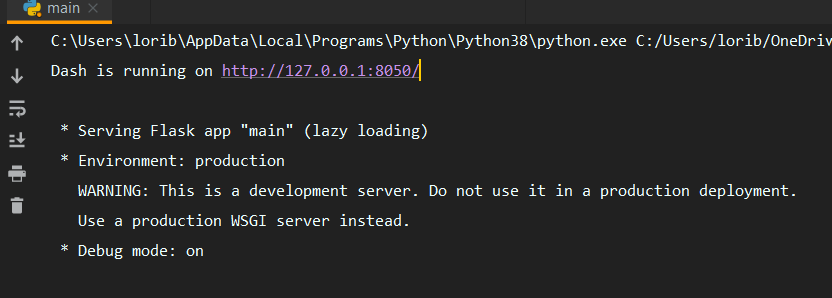
\includegraphics[width=300pt]{console.png}
        \caption{Console Output}
    \end{figure}

    This will take you to the Dash webpage we created where you can view and interact with the visualizations. Our main interaction is being able to adjust the 2 sliders underneath the map we created to see how the data points change at a specific year, or with a predetermined sea level input. \\
    \begin{figure}[h]
        \centering
        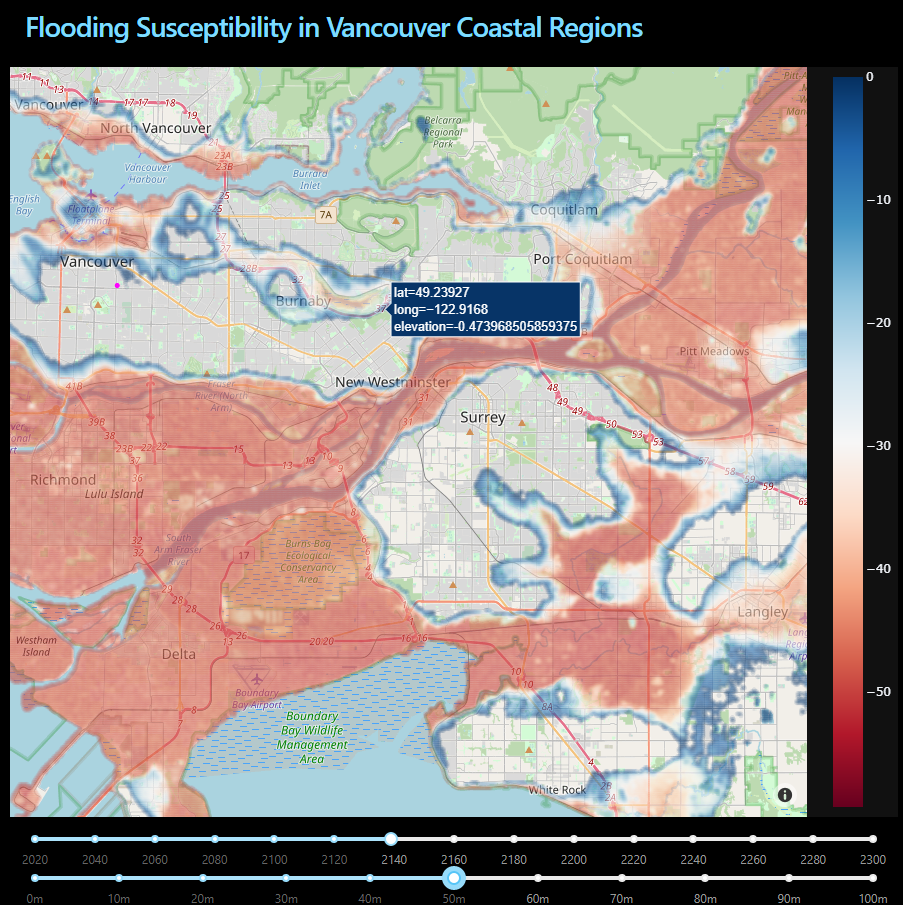
\includegraphics[width=300pt]{frontend.png}
        \caption{Front-end Output}
    \end{figure}


    \section*{Project Changes}
    \hspace{\parindent}Based on the feedback received from our proposal, we have made some minor changes to our project plan to streamline the process. For example we realized the vagueness of our original research question and thus adjusted it to be more focused by specifying a certain time period to analyze. We also realized the repetitiveness in only performing a linear regression calculation on our data seeing as we have done the same thing on Assignment 1. After this was brought to our attention, we looked into other methods to model our calculated data and decided on a Theil-Sen regression and SARIMAX prediction model. The Theil-Sen regression is what determines our predictions but the SARIMAX model provides a nice moving average prediction model for visualization. We also realized the complexity of having a dropdown menu and other forms of interactive output, due to our limited expertise in front-end development. We stuck to having 2 sliders, one for the year and one for the sea level and a color bar which determines flood severity based on elevation.


    \section*{Discussion}
    \hspace{\parindent}Our computational exploration does a sufficient job in answering which coastal areas in Vancouver are the most susceptible for flooding 280 years into the future. This is displayed by our mapbox visualization and data interpretation of the annual mean sea level changes. If we move the slider all the way to 2300, we can see which areas are going to be the most impacted, due to the greater frequency of data points which are below sea level. By analyzing this map we see that the most heavily impacted areas are the coastlines around Richmond, Delta, and Surrey, due to their lower elevations. With the second slider, the user can select a predetermined sea level and see which areas will be affected with that particular sea level. \\

    Additionally, our graphical models display the changes in sea levels over the years. We can see that there is a positively increasing trend, which means that due to the increasing temperatures in our climate the sea levels are in fact beginning to rise. Our predicted model shows how high the changes will be in the future, urging us as Earth’s inhabitants to take action in order to minimize this trend. \\

    One of the main limitations was with finding an appropriate dataset for the sea level changes. It was very hard to find a dataset that was in a format that would be easily interpreted by our program, hence the many data filtrations/transformations we needed to apply to this dataset. It was also hard to find a dataset that dates back to an earlier year in the past, as in earlier than 1992. This affects our prediction model because the model was trained over a shorter period of time, so the projected trend may be less extreme than it is in reality. \\

    Another limitation was with the plotly library, some of the functions were difficult to use because some parameters for our figures wouldn’t work as desired or described in the documentations, so we needed to research workarounds for these issues using other functions, which consumed a lot of time of the project. However, researching documentations for modules and seeking solutions for errors online is very typical in a software engineering environment, so it was good for us to get this experience. We used dash to display our plotly figures, the main challenge from this was dealing with the front end components. Since we are not experienced with front end development it was quite difficult to work with the dash framework, which results in an interactive display that is more basic than we intended. However, we still made an effort to research how to work with this framework and were able to implement a slider which provides an interactive experience with our figures. \\

    The main obstacle we faced in designing this program was implementing the prediction model algorithm. This was difficult because it was hard to find a model that was appropriate for our situation. We also wanted to implement this algorithm without as much help from an external library as possible, to increase the complexity of our calculations. We used a Theil-Sen regression to determine the predicted sea levels, but also have a SARIMAX prediction model for a more complex prediction visualization. \\

    The next steps for our exploration would be to incorporate temperature data as well for a stronger analysis. If we displayed figures with temperature against sea level rise we would be able to see the relationship between climate change and sea level rise directly, rather than assuming it as background knowledge. If we used the relationship between global temperature change and sea level change to train our prediction model rather than sea level change and time, maybe our model would have been more accurate. \\

    In conclusion, our computational exploration allows us to see the coastal areas in the Vancouver region most susceptible to flooding up to 280 years into the future, due to our trained prediction model computations, data interpretations, and geographical visualizations, despite the challenges and limitations faced.


    \section*{References}
    \begin{hangparas}{.25in}{1}
        Canada, N. (2020, October 16). Government of Canada. Retrieved November 06, 2020, from \\ https://www.nrcan.gc.ca/topographic-information/10785 \\

        Bhattiprolu, Sreenivas. “163 - An Introduction to Time Series Forecasting - Part 3 Using ARIMA in Python.” YouTube,
        YouTube, 1 Oct. 2020, www.youtube.com/watch?v=TSfdvQ0ARwI \\

        Brownlee, Jason. How to Create an ARIMA Model for Time Series Forecasting in Python, 9 Jan. 2017, \\
        http://machinelearningmastery.com/arima-for-time-series-forecasting-with-python/ \\

        Dash Documentation & User Guide. (n.d.). Retrieved December 13, 2020, from https://dash.plotly.com/ \\

        Explainer: How climate change is accelerating sea level rise. (2019, September 30). Retrieved November 05, 2020, from https://www.carbonbrief.org/explainer-how-climate-change-is-accelerating-sea-level-rise \\

        Kulp, S., & Strauss, B. (2019, October 29). New elevation data triple estimates of global vulnerability to sea-level rise and coastal flooding. Retrieved November 05, 2020, from https://www.nature.com/articles/s41467-019-12808-z \\

        Laboratory for Satellite Altimetry / Sea Level Rise. (n.d.).
        Retrieved November 06, 2020, from \\ https://www.star.nesdis.noaa.gov/socd/lsa/SeaLevelRise/LSA\_SLR\_timeseries.php \\

        Little, S. (2019, November 01). Sea level rise may be '3 times worse' than expected. Here's how it could impact Metro Vancouver. Retrieved November 05, 2020, from https://globalnews.ca/news/6102304/sea-level-rise-metro-vancouver/\\

        (n.d.). Retrieved December 13, 2020, from https://numpy.org/doc/ \\

        Pandas. (n.d.). Retrieved December 13, 2020, from https://pandas.pydata.org/ \\

        Plotly Python Graphing Library. (n.d.). Retrieved November 05, 2020, from https://plotly.com/python/ \\

        Report: Flooded Future: Global vulnerability to sea level rise worse than previously understood. (2019, October 29). Retrieved November 06, 2020, from https://www.climatecentral.org/news/report-flooded-future-global-vulnerability-to-sea-level-rise-worse-than-previously-understood \\

        Rising Sea Levels Threaten to Flood Southern Vietnam by 2100. (n.d.). Retrieved December 13, 2020, from https://www.voanews.com/east-asia-pacific/rising-sea-levels-threaten-flood-southern-vietnam-2100 \\

        SciPy. (n.d.). Retrieved December 13, 2020, from
        https://docs.scipy.org/doc/scipy/reference/ \\

        Vancouver has the highest population density in Canada: Census. (2017, December 28). Retrieved November 05, 2020, from https://biv.com/article/2017/02/vancouver-has-highest-population-density-canada-ce

    \end{hangparas}


\end{document}
